%
% ..............................................................................
\section{Implementation and use of GMPEs in seismic hazard analysis}
The \gls{acr:oqe} contains a large set of \glspl{acr:gsim}
developed for different tectonic regions. 
%
Currently the engine includes \glspl{acr:gsim} for shallow earthquakes
in active tectonic regions, earthquakes in stable continental regions,
subduction regions and geothermal areas.

\glspl{acr:gsim} are implemented following a template model (in the 
Python jargon a base class) which defines the basic behaviour and 
describes the principles to be followed for their implementation.
%
Each \gls{acr:gsim} contains a definition of the independent parameters
used to describe the rupture, the site conditions, the rupture-site
distance metrics, the intensity measure types supported, the type of 
standard deviation provided, the tectonic region where the use of the 
\gls{acr:gsim} is recommended.

The main advantage of this approach is that \glspl{acr:gsim}, no matter 
which are their specific properties or features, behave following 
a common standard. 
%
For example, this feature allowed the creation on top of the 
\gls{acr:gsim} library of a universal testing procedure, a standard 
applied to all the models implemented in the \gls{acr:oqe} which 
guarantees a baseline uniform quality assurance level. 

A second advantage of the developed library relates to its flexibility 
and modularity. Once the properties of main objects are defined, 
\glspl{acr:gsim} can be used interchangeably. 
%
For example, the OpenQuake Ground Motion Toolkit 
\parencite{weatherill2014} builds on top of this library and 
includes tools for computing residuals given a dataset 
of recordings, or for the calculation of trellis plots that compare the scaling of multiple GMPEs side by side in terms of magnitude, distance, site-condition, spectra etc..
%
Figure \ref{fig:gsim_mag_scaling} shows the scaling of ground-motion 
versus magnitude for some of the \glspl{acr:gsim} implemented in the 
\gls{acr:oqe}.
%
The ground motion is computed for a site at a R$_{jb}$ distance of 
about 33 km with V$_{S,30}$ equal to 760 m/s from a rupture with a 
strike of dip of 45 degrees toward south for two different values 
of rake (i.e. rupture mechanism). The upper panel of Figure 
\ref{fig:gsim_mag_scaling} shows the position of the site and 
the rupture.
% . . . . . . . . . . . . . . . . . . . . . . . . . . . . . . . . . . . > Figure
\begin{figure}[hb]
\centering
% left bottom right top
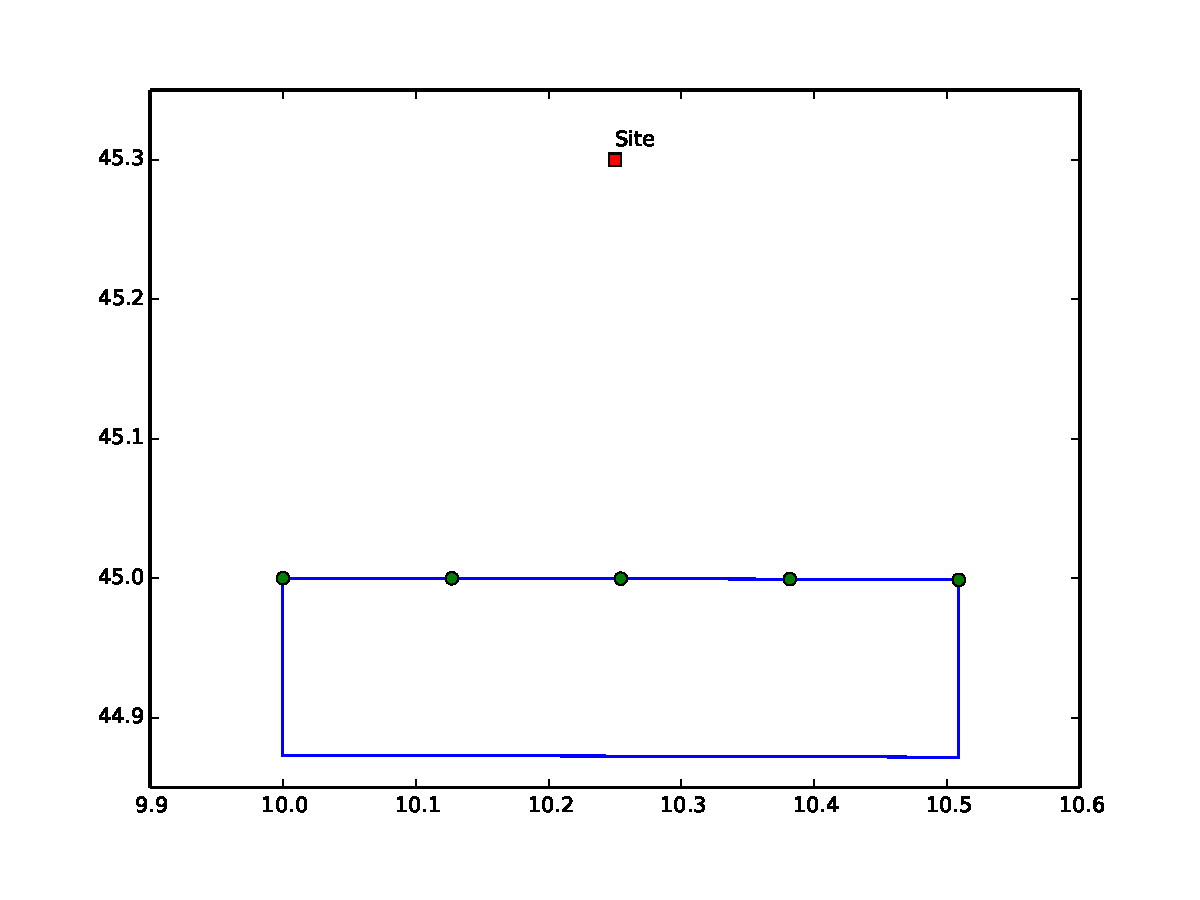
\includegraphics[width=10cm]{./Pictures/gsim/rupture_plot.pdf}
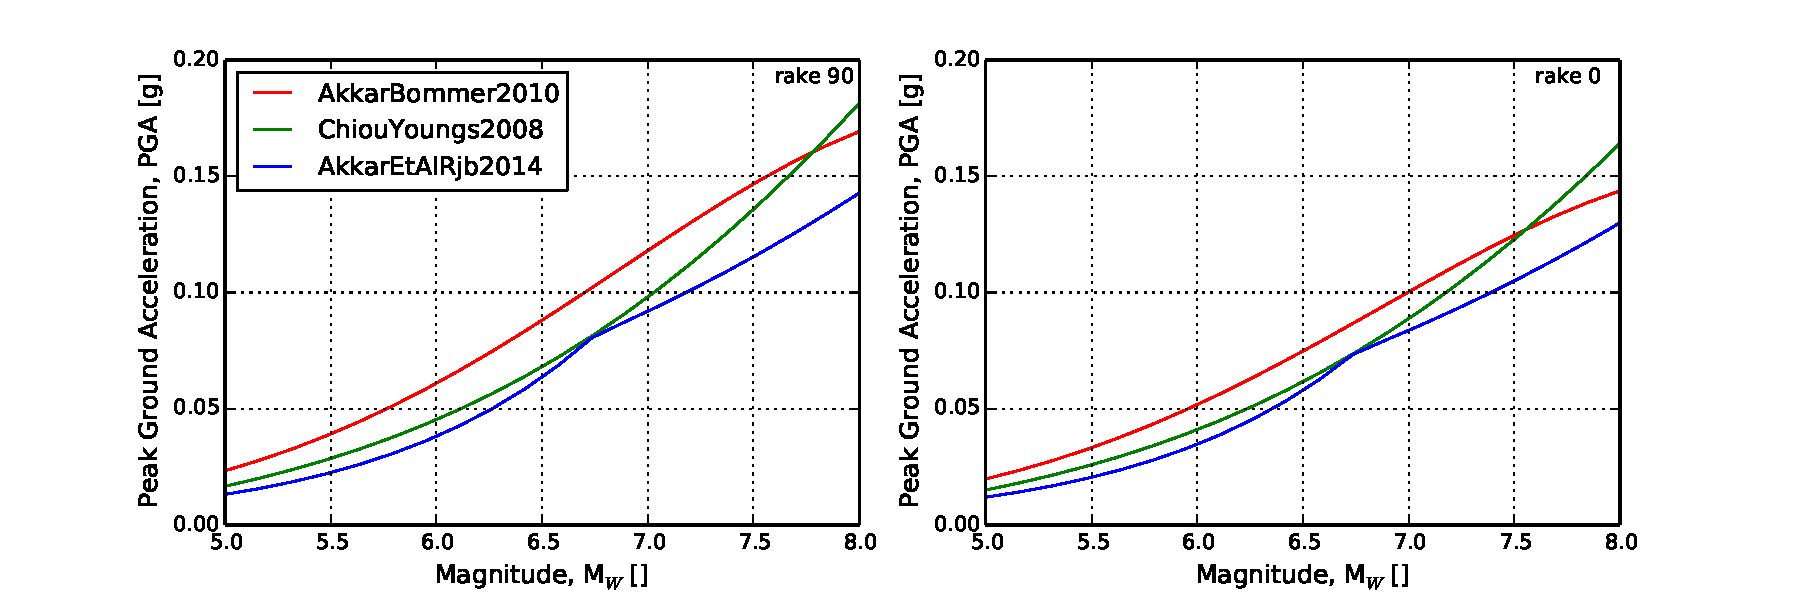
\includegraphics[trim = 23mm 0mm 23mm 5mm, clip, width=\textwidth]
    {./Pictures/gsim/mag_scaling_example.pdf}
    \caption{
        (upper panel)
        Simple schematic with the surface projection of the 
        rupture and the site (red square) used in this example. 
        The green dots show the position of the top of rupture.
        (lower panels)
        Scaling of Peak Ground Acceleration as a function 
        of magnitude obtained by some of the \gls{acr:gsim} 
        implemented in the \gls{acr:oqe}. 
    }
\label{fig:gsim_mag_scaling}
\end{figure}
% . . . . . . . . . . . . . . . . . . . . . . . . . . . . . . . . . . . < Figure
%
% . . . . . . . . . . . . . . . . . . . . . . . . . . . . . . . . . . . . . . .
\subsection{Testing}
%
The progressively increasing complexity of 
\glspl{groundshakingintensitymodel}
is giving more and more emphasis and relevance to the validation 
of results provided by the \gls{acr:gsim} implemented within 
\gls{acr:psha} codes and the results of original \gls{acr:gsim} 
implementations as described in the scientific literature 
(or directly provided by the authors).

The standard process adopted for the implementation in the 
\gls{acr:oqe} of a \gls{groundshakingintensitymodel} requires a 
set of verification tables each one containing values of 
ground-motion (or standard deviation) computed using a large 
number of combinations of the predictor variables. 
%
Table \ref{tab:verification} shows a simplified example of a 
\gls{acr:gsim} verification table; it consists of: a header 
line with (standard) names for each of the column, a number
of lines each one containing values of the predictor variables
plus the computed values of ground-motion intensity or standard
deviation.
% --------------------------------------------------------------------->>> Table
\begin{table}[!ht]
\centering
\caption{Schematic of a \gls{acr:gsim} verification table used in the 
\gls{acr:oqe}.}
\begin{tabular}{|cccccc|}
\hline
\rowcolor{anti-flashwhite}
M & R & V$_{S,30}$ & IMT$_1$ & IMT$_2$ & ... \\
\hline 
val$_{1,1}$ & val$_{1,2}$ & val$_{1,3}$ & val$_{1,4}$ & val$_{1,5}$ & \\
val$_{2,1}$ & val$_{2,2}$ & val$_{2,3}$ & val$_{2,4}$ & val$_{2,5}$ & \\
... & & & & & \\
\hline
\end{tabular}
\label{tab:verification}
\end{table}
% ---------------------------------------------------------------------<<< Table
Examples of verification tables are available on the OpenQuake-hazardlib Github
repository\footnote{
\href{https://github.com/gem/oq-hazardlib/tree/master/openquake/hazardlib/tests/gsim/data}{
https://github.com/gem/oq-hazardlib/tree/master/openquake/hazardlib/tests/gsim/data}
}.

Using these tables and an automated verification procedure implemented
in the \gls{acr:oqe}, it is possible to verify the consistency between 
the original results and the corresponding values computed with the 
version of the \gls{acr:gsim} implemented. 
%
On average we accept \gls{acr:oqe}

GEM recommends contextually to the publication of \gls{acr:gsim}
distributing as an electronic attachment the table of coefficients as well 
as of a set of verification tables (or a software which allows the generation 
of these tables). This can certainly improve the reproducibility of the 
new models proposed and most of all would improve the quality and 
robustness of the computed hazard.
%
% . . . . . . . . . . . . . . . . . . . . . . . . . . . . . . . . . . . . . . .
\subsection{Selection criteria}
%The \gls{acr:oqe} does not provide tools supporting a formal \gls{acr:gsim}
%selection process, which is now common practice in a PSHA model building 
%process \parencite[see for example][]{delavaud2012}. 
%
%Nevertheless, in order to ensure the higher level of consistency between 
%the selection procedure and the calculation of hazard it is recommendable 
%to use in both the phases the same \gls{acr:gsim}. 
This section will be completed later.
%
% . . . . . . . . . . . . . . . . . . . . . . . . . . . . . . . . . . . . . . .
\subsection{Spatial correlation of ground motion}
This section will be completed later.
